In this chapter, the systematic uncertainties relevant for neutrino
induced single photon production are detailed.

The systematic uncertainties are divided according to their
sources. Similarly to most of the \Gls{ND} cross section analysis,
they reduce to flux (Section~\ref{sec:fluxsyst}), cross section
(Section~\ref{sec:xsecsyst}) and detector (Section~\ref{sec:detsyst})
systematic errors. Additionally, the statistical uncertainty and the
efficiency uncertainty are also taken into account.

However, given the scale of the contamination of events that happened
outside the Fiducial Volume (\Gls{OOFV}) of the \Gls{FGD}1 and the
expected differences which arise for the systematic uncertainty when
considering neutrino interaction happening in the \Gls{FGD}1 and the
rest of the detector, the two backgrounds systematic uncertainties are
independently motivated.

Finally, all the systematic uncertainties are combined and summarised
in Section \ref{sec:totaluncertainty}.

\clearpage

\section{Flux systematic uncertainties}
\label{sec:fluxsyst}

The flux systematic error accounts for the uncertainty one has in
predicting the flux of neutrinos. The uncertainty was propagated using
a code called \texttt{\Gls{JReWeight}} (see instructions and
references in \cite{t2kreweight}), which changes the relative
importance of the selected events based on the neutrino energy and
according to the relative uncertainty as shown in
Figure~\ref{fig:fluxsystematics}. Note that these errors are very
correlated; although there are 100 bins of energy for the neutrino,
after decomposition of the covariance matrix, only seven parameter
eigenvalues are greater than $1\%$, which indicates that the flux
error can been parametrised by only few parameters. These are, by
decreasing order of importance:
\begin{itemize}[noitemsep,topsep=0pt]
\item the proton interaction error, which are constrained by the
  NA61~/~SHINE
  experiments~\cite{Abgrall:2011ae,Abgrall:2011ts,Abgrall:2015hmv},
\item the beam characteristic (profile, intensity, direction) which
  are characterised {\it in situ}, as shown in
  Section~\ref{sec:t2kbeamline},
\item the survey of material around the target station,
\item the horn current and positions.
\end{itemize}

\begin{figure}[ht]
  \center
  \includegraphics[width=0.8\textwidth]{T2K-TN-254/images/systematics/Flux.pdf} \\
  \includegraphics[width=0.8\textwidth]{T2K-TN-254/images/systematics/DiagError.pdf}
  \caption[T2K flux uncertainty and correlations across true energy
  bins in at ND280 and at SK]{\textbf{\textit{Top:}} The \Gls{TK} flux
    uncertainty correlations across true energy bins in for \Gls{ND}
    and \Gls{SK}, while running in \Gls{FHC} and \Gls{RHC} modes, for
    \Gls{numu}, \Gls{anumu}, \Gls{nue} and \Gls{anue}.
    \textbf{\textit{Bottom:}} The diagonal uncertainty for \Gls{numu}
    neutrinos in \Gls{FHC} at the \Gls{ND}. Both extracted from
    \Gls{TK} beam working group
    inputs~\cite{TomislavVladisavljevicFluxTuning2017,MarkHartzFluxUncertainty2017}.}
  \label{fig:fluxsystematics}
\end{figure}

As can be seen in Figure~\ref{fig:fluxsystematics}, the flux
uncertainty is expected to be around $10\%$.

Note that the flux uncertainty was constructed for \Gls{FGD} neutrino
interactions. The photons, on the other hand, can come from regions
far from the \Gls{FGD} central region. Following what was done in
\cite{MarkScott2013}, the conclusion was that the error should not be
increased by more than $5\%$ for \Gls{ECal} interactions. The increase
of the error is considered negligible compared to other effects taken
into account here.

Another motivation for not inflating the flux error is that the
photons do not come from very far from the tracker region, as can be
seen in Appendix~\ref{app:oofvphoton}. The conversion length of the
photons in the \Gls{ECal} ($10.4\text{~cm}$) is much shorter than for
a standard scintillator ($41.1\text{~cm}$), so it is not expected
that the \Gls{OOFV} neutrino interactions come from far regions such
as the \Gls{SMRD}.

The \Gls{PDF} (for Probability Density Function) of the number of
selected events is shown in Figure~\ref{fig:fluxsystematicspdf}.

\begin{figure}[ht]
  \begin{adjustbox}{center}
    \includegraphics[width=0.8\textwidth]{images/NCg/Flux.pdf} 
  \end{adjustbox}
  \caption[Effect of the flux uncertainty on the number of selected
  events]{Effect of the flux uncertainty on the number of selected
    events. The nominal central value for \Gls{MC} is indicated by the
    arrow.}
  \label{fig:fluxsystematicspdf}
\end{figure}


%%% Local Variables:
%%% mode: latex
%%% TeX-master: "Thesis"
%%% End:
\clearpage

\section{Cross section systematic uncertainties}
\label{sec:xsecsyst}

The cross section uncertainties were propagated using the
\texttt{\Gls{T2KReWeight}} package~\cite{t2kreweight}, which modifies
the relative importance of the neutrino events based on a change of the
underlying cross section model.

\subsection{Cross section uncertainty on primary processes}
\label{subsec:primaryprocessuncertainty}
In this section, the cross section uncertainties on primary processes
are explained. The main background of the analysis comes from \gls{piz}
\Gls{NC} \Gls{RES} (resonant) interactions. There are a lot of vetoes
in the selection which remove muons from charged current interactions
and the second decay photons from the \Gls{piz}. All the cross section
systematic errors propagated are the same as those that were recently
used for the near detector fits supporting the oscillation analysis
in~\cite{Abe:2017vif} and in Chapter~\ref{chap:banff}.

Even if the \Gls{CCQE} processes are dominant at \Gls{TK} energies,
their impact on the analysis is minimal, since they only contribute
marginally to the selection of events as can be seen in
Table~\ref{tab:reaction}, standard cross section errors were
nevertheless propagated and will be explained here.

\subsubsection{Free nucleon resonant interaction uncertainties}
\label{subsubsec:freeres}
There are three uncertainties related to the \Gls{RES}
interactions. All of them are parameters of the Rein and Sehgal
model~\cite{Rein1,Rein2}.

\paragraph{Resonant axial mass}
This parameter controls the axial mass ($M_A^{\text{RES}}$). This is
one of the fundamental inputs for the cross section calculation
related to the form factor. \Gls{TK} now uses a new form factor
compared to the original one from Rein and Sehgal, which has the
form~\cite{PhysRevD.77.053001}:
\begin{equation}
  \label{eq:ffres}
  \sigma_{\text{RES}} \propto  C^A_5(Q^2)=\frac{C^A_5(0)}{\left(1+\frac{Q^2}{\left.M_A^{\text{RES}}\right.^2}\right)^2}.
\end{equation}
Where the linear dependence of the neutrino cross section
($\sigma_{\text{RES}}$) to the axial form factor ($C^A_5$) is made
explicit. In this equation, $M_A^{\text{RES}}$ is the axial mass
(which is the equivalent for \Gls{RES} cross section to the \Gls{CCQE}
$M_A^{\text{QE}}$ described in Section~\ref{subsec:ccqe}), and $Q^2$
(see Footnote~\ref{ftn:qsquare} on page~\pageref{ftn:qsquare}) is the
momentum transfer.

\paragraph{Resonant axial form factor at \texorpdfstring{$Q^2=0$}{TEXT}}
In Equation~\ref{eq:ffres}, the parameter $C^A_5(0)$ is also an
uncertainty, which acts on the total normalisation of the \Gls{RES}
events.

\paragraph{Isospin 1/2 background} The background component refers to
the non-resonant component contribution of the cross section as
described in Section~\ref{subsec:res}.

\paragraph{Tuning and uncertainty}
Several tunings of these parameters are done using different
combinations of the available data (bubble chamber), and using
channels that are sensitive or not to the background
term~\cite{TN315}.

The errors used are listed in Table~\ref{tab:reserror}.

\begin{table}[ht]
  \begin{adjustbox}{center}
    \begin{tabular}{cccccc}
      \toprule
      Parameter & Value & Error & \multicolumn{3}{c}{Correlation} \\
                &       &       & $M_A$   & $C_5^A$ & $I_{1/2}$ \\
      \midrule
      $M_A$     & 1.07  & 0.15  & $1$     & $-0.83$ & $-0.01$   \\
      $C_5^A$   & 0.96  & 0.15  & $-0.83$ & $1$     & $-0.31$   \\
      $I_{1/2}$ & 0.96  & 0.40  & $-0.01$ & $-0.31$ & $1$       \\
      \bottomrule
    \end{tabular}
  \end{adjustbox}
  \caption[Neutrino RES error used in the analysis]{Neutrino \Gls{RES}
    errors used in the analysis, reproduced from~\cite{TN315}.}
  \label{tab:reserror}
\end{table}

\subsubsection{Nuclear resonant interaction uncertainty, the
  \Gls{MiniBooNE} \texorpdfstring{$NC1\pi^{0}$}{TEXT} fits}
\label{subpar:miniboonefits}
Due to the relative importance of \Gls{piz} in the analysis, it was
decided to add additional parameters to properly deal with the
uncertainties coming from these events where a \piz was created. It
should be noted that most of these backgrounds are from resonant
interactions and single \Gls{piz} production as can be seen in the
previous section
(Tables~\ref{tab:reaction}~and~\ref{tab:topo}). Furthermore, in
Figures~\ref{fig:pizeff1}~and~\ref{fig:pizeff2}, one can see that the
efficiency in selecting these \Gls{piz} from resonant interactions is
not flat.  Therefore, any uncertainty on the \Gls{piz} background that
creates a shape difference in the pion kinetic space is expected to
have a significant importance in the overall systematic error
budget. These parameters are relevant since none of the previously
described parameters has the ability to change the pion momentum
distribution. This can be seen in Figure~\ref{fig:currenterrors},
where the neutral pion (\Gls{piz}) measurement was from
\Gls{MiniBooNE}~\cite{AguilarArevalo:2009ww} and compared to the
\Gls{NEUT} prediction and errors.

Based on this study, two parameters were re-introduced from cross
section parametrisation (identical to the ones used in Section B.3
of~\cite{T2KLong}). The reason is that the errors on the pion
kinematics produced by the cross section parameter described earlier
do not cover all the data points and a shape discrepancy can be
seen. Note that all the plots and studies were realised with the
newly-released \Gls{NUISANCE}~\cite{NUISANCE2017}.

The \Gls{TK} pion model (which is the Rein and Sehgal
model~\cite{Rein1,Rein2} with the parameters: axial mass,
normalisation of the form factor and isoscalar background free) is
fitted using the bubble chamber data, and the reasons why this
under-coverage could happen are multiple: for example a problem with
\Gls{FSI}, but also the Pion-less Delta decay or any other nuclear
effects (such as the one discussed in the Section~\ref{subsec:res})
that makes the extrapolation from a single nucleon to nuclear target
wrong. Note that all the parameters described above are designed to
act on the leading muon kinematics in the Charged Current resonant
channels.

In most of the extended models that deal with resonant interactions in
nuclear media, the modifications that arise are dependent on the
momentum of the resonance (Delta width), so a parameter that modifies
the shape of the $W$ distribution is a fairly natural way to account
for differences arising from nuclear correction. The parameters as
function of $Q^2$ have more impact on the leading lepton. If one looks
at the pion momentum, these parameters are acting as normalisation and
cannot change the shape of the pion momentum.

For the purpose of the analysis, the \Gls{MiniBooNE} \Gls{NC}\gls{piz}
momentum distribution~\cite{AguilarArevalo:2009ww} was fitted using
the Delta width and position of the Breit-Wigner distribution.

In the \Gls{MiniBooNE} fits, the normalisation of the data is left
free as most of the existing bubble chamber data are already
constraining the normalisation of the nucleon level resonant processes
and were explicitly tuned to accommodate other \Gls{MiniBooNE}
\Gls{CC} and \Gls{NC} measurement normalisations~\cite{TN315}.

Similarly, the \Gls{FSI} (for which the systematic error effects are
not displayed in any of the plots in this section) can also change the
normalisation (but not the shape of the pion momentum). This is
because it is not simple to code a reweighting scheme which changes
the shape of the kinematics of the pions when they undergo the
\Gls{FSI}. Therefore, given that the normalisation of the data is a
convolution of a number of non trivial parameters, it was chosen to
leave the normalisation free, and the aim of this fit is solely to be
able to reproduce \Gls{MiniBooNE} pion kinetical shape with sensible
errors.

After doing the fit, one gets the result for the parameters listed in
Table~\ref{tab:fitresult}. In this case, only the two Delta parameters
were fitted, while the other parameters were fixed at their initial
tuned values.

\begin{table}[ht]
  \begin{adjustbox}{center}
    \begin{tabular}{ccc}
      \toprule
      Parameter & Prior & Uncertainty \\
      \midrule
      $\Delta$ mass mean  & -0.002 & 0.004 \\
      $\Delta$ mass width & -0.26  & 0.14  \\
      \bottomrule
    \end{tabular}
  \end{adjustbox}
  \caption[MiniBooNE $p_{NC\pi^{0}}$ shape-only fit
  result]{\Gls{MiniBooNE} $p_{NC\pi^{0}}$ shape-only fit result.}
  \label{tab:fitresult}
\end{table}

The plots in Figure~\ref{fig:miniboonepostfit} show the error coverage
one gets after generating toy with the errors from
Table~\ref{tab:fitresult} and the all the standard errors
from~\cite{TN193}. The Figure~\ref{fig:miniboonepostfitcoh} shows the
same distribution with an increased \Gls{NC} coherent uncertainty from
$30\%$ to $100\%$. This was done to try to accommodate data~/~\Gls{MC}
differences in the forward region, which is expected to be purer in
coherent interactions as illustrated on
Figure~\ref{fig:miniboonebreakdown}.


\begin{figure}[ht]
  \center
  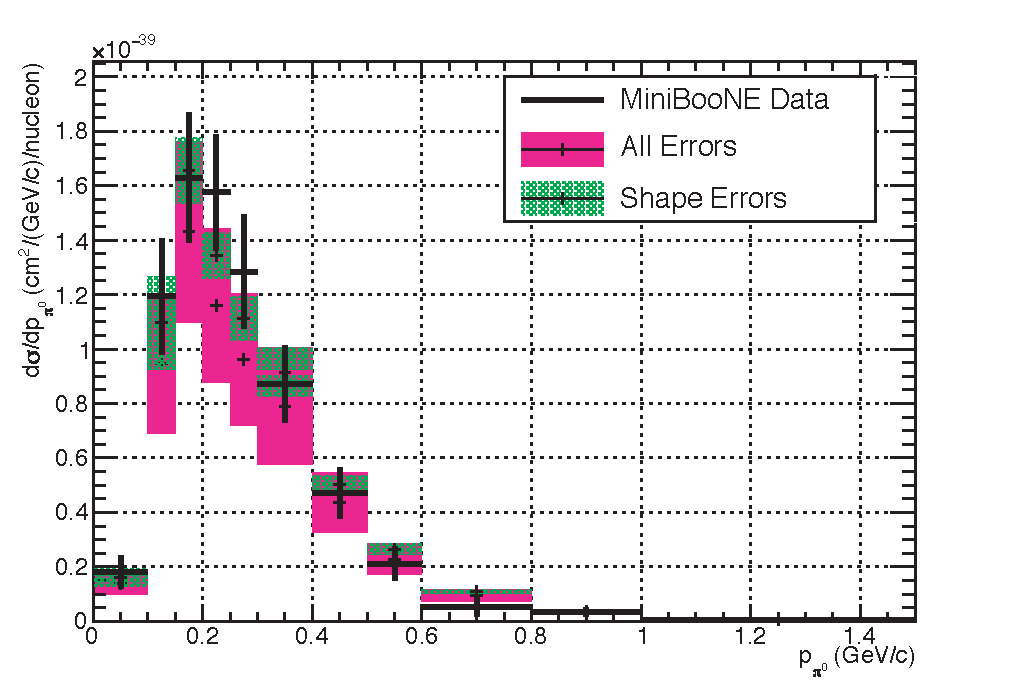
\includegraphics[width=0.8\textwidth]{T2K-TN-254/images/systematics/MB_NC1Pi0_pPi0_nu_curr_good.pdf}\\ %%
  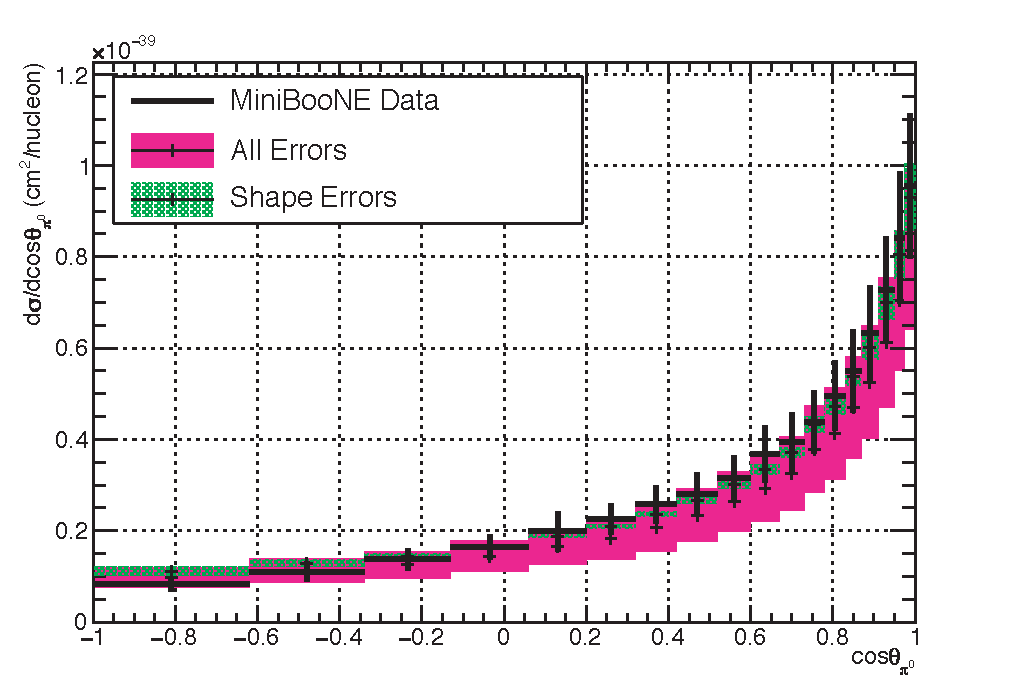
\includegraphics[width=0.8\textwidth]{T2K-TN-254/images/systematics/MB_NC1Pi0_ctPi0_nu_curr_good.pdf} %%
  \caption[MiniBooNE error coverage from current
  parametrisation]{\Gls{MiniBooNE} error coverage from standard
    parametrisation~\cite{TN315} (Table~\ref{tab:reserror}). The black
    line shows the \Gls{MiniBooNE} neutrino mode \Gls{NC}\gls{piz}
    data~\cite{AguilarArevalo:2009ww}, magenta boxes \Gls{NEUT}
    predictions with errors, overlayed green boxes are shape only
    variations from \Gls{NEUT}. \textbf{\textit{Top:}} Pion momentum
    distribution. \textbf{\textit{Bottom:}} Pion angular
    distribution.}
  \label{fig:currenterrors}
\end{figure}

\begin{figure}[ht]
  \center
  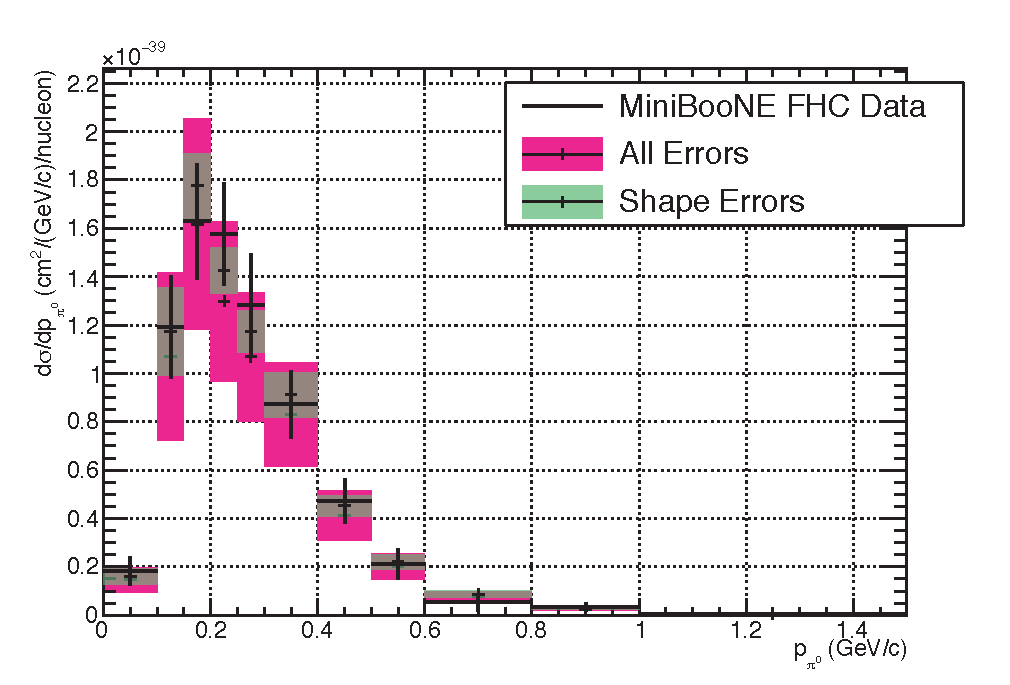
\includegraphics[width=0.8\textwidth]{T2K-TN-254/images/systematics/MB_NC1pi0_1Dppi0_fhc_nu_1WShape_good.pdf}\\ %%
  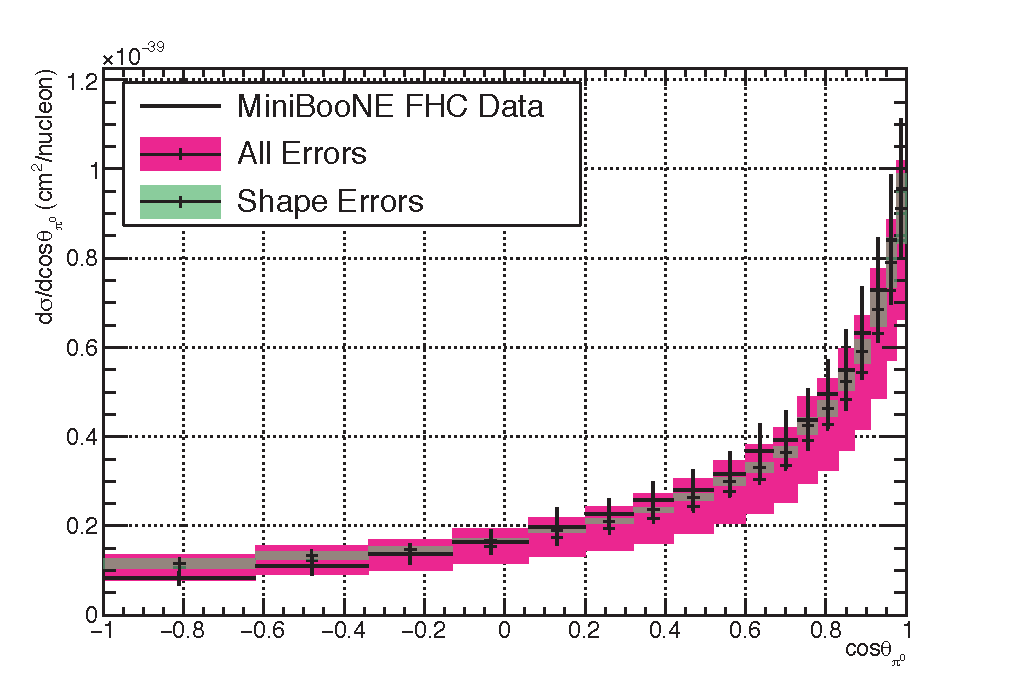
\includegraphics[width=0.8\textwidth]{T2K-TN-254/images/systematics/MB_NC1pi0_1Dcospi0_fhc_nu_1WShape_good.pdf} %%
  \caption[MiniBooNE error coverage using the fitted
  errors]{\Gls{MiniBooNE} error coverage using the fitted errors from
    standard parametrisation~\cite{TN315} (Table~\ref{tab:reserror})
    and $W$-shape error (Table~\ref{tab:fitresult}). The black line
    shows the \Gls{MiniBooNE} neutrino mode \Gls{NC}\gls{piz}
    data~\cite{AguilarArevalo:2009ww}, magenta boxes \Gls{NEUT}
    predictions with errors, overlayed green boxes are shape only
    variations from \Gls{NEUT}. \textbf{\textit{Top:}} Pion momentum
    distribution. \textbf{\textit{Bottom:}} Pion angular
    distribution.}
  \label{fig:miniboonepostfit}
\end{figure}


\begin{figure}[ht]
  \center
  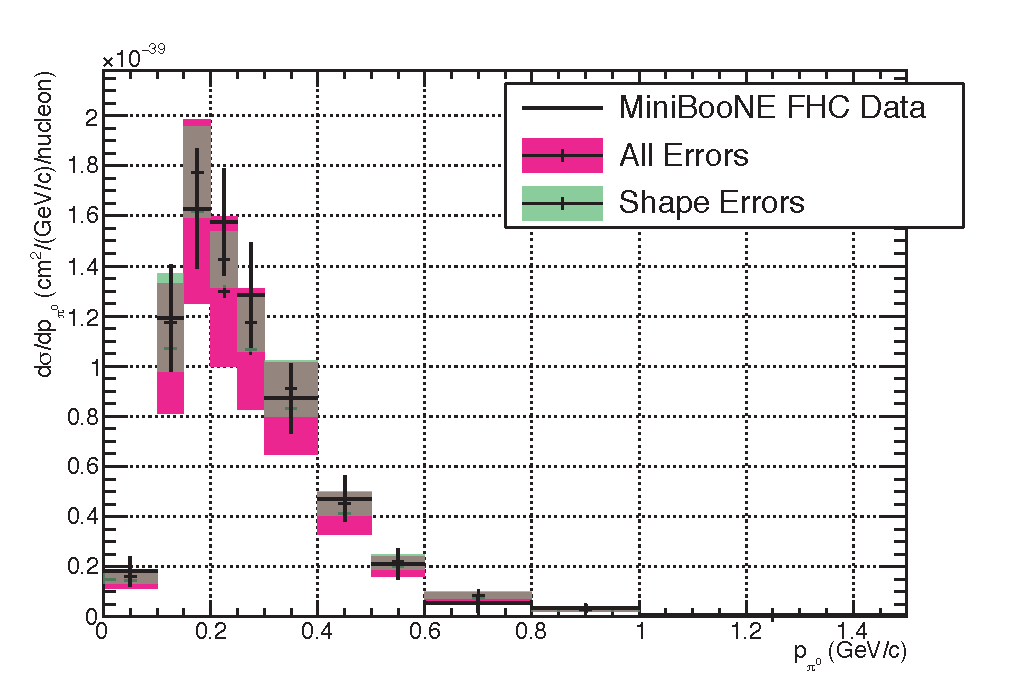
\includegraphics[width=0.8\textwidth]{T2K-TN-254/images/systematics/MB_NC1pi0_1Dppi0_fhc_nu_1WShape_highNCCoh_good.pdf} \\ %%
  \includegraphics[width=0.8\textwidth]{T2K-TN-254/images/systematics/MB_NC1pi0_1Dcospi0_fhc_nu_1WShape_highNCCoh_good.pdf} %%
  \caption[MiniBooNE error coverage using the fitted errors and an
  additional error for NC COH events]{\Gls{MiniBooNE} error coverage
    using the fitted errors from standard parametrisation~\cite{TN315}
    (Table~\ref{tab:reserror}) and from $W$-shape error
    (Table~\ref{tab:fitresult}) with a $100\%$ error on \Gls{NC}
    coherent interaction The black line shows the \Gls{MiniBooNE}
    neutrino mode \Gls{NC}\gls{piz} data~\cite{AguilarArevalo:2009ww},
    magenta boxes \Gls{NEUT} predictions with errors, overlayed green
    boxes are shape only variations from
    \Gls{NEUT}. \textbf{\textit{Top:}} Pion momentum
    distribution. \textbf{\textit{Bottom:}} Pion angular
    distribution.}
  \label{fig:miniboonepostfitcoh}
\end{figure}

\begin{figure}[ht]
  \center
  \includegraphics[width=0.8\textwidth]{T2K-TN-254/images/systematics/MB_NC1Pi0_comp_ppi.pdf} %%
  \includegraphics[width=0.8\textwidth]{T2K-TN-254/images/systematics/MB_NC1Pi0_comp_cospi.pdf} %%
  \caption[MiniBooNE NC$\pi^0$ differential
  distribution]{\Gls{MiniBooNE} \Gls{NC}\gls{piz} differential
    distribution, top: $p_{\pi^{0}}$, bottom:
    $\cos(\theta_{\pi^{0}})$, broken down by \Gls{NEUT} reaction
    modes, the central values and are the same as for
    \ref{fig:miniboonepostfitcoh}.}
  \label{fig:miniboonebreakdown}
\end{figure}

In the case of the \Gls{OOFV} background interactions, they mostly are
from \Gls{RES} interactions, as can be seen in
Tables~\ref{tab:reaction}~and~\ref{tab:target}. The same effects as
described before are also valid so one could wonder if having a carbon
measurement is enough. However, given that there is no
\Gls{NC}\gls{piz} measurement on target other than carbon (and Argon
with \Gls{ArgoNeuT}~\cite{Acciarri:2015ncl}) where the \Gls{piz}
kinematics are available, and the size of the detector error, it was
considered that the differences in uncertainty between carbon and
other nuclear targets should be negligible and thus the uncertainties
described above were applied to the \Gls{OOFV} interactions.

\clearpage

\subsubsection{Relativistic Fermi Gas parameters}
The \Gls{RFG} model is dependent on two fundamental parameters. Both
of them can be determined via electron
scattering~\cite{Alvarez-Ruso:2017oui}.

The first parameter is the Fermi momentum, this quantity is determined
by the width of the elastic peak. The second parameter is the binding
energy, which is determined by the position of the elastic peak. This
quantity corresponds to the energy needed to extract a nucleon from
the Fermi sea.

Unfortunately, even with very accurate electron scattering
measurements, it is hard to find values for these two parameters which
can explain all the electron scattering data~\cite{TN315}, indicating
a deficiency in the model.

The values and uncertainties that are used at \Gls{TK} are listed in
Table~\ref{tab:rfgerror}

\begin{table}[ht]
  \begin{adjustbox}{center}
    \begin{tabular}{cccc}
      \toprule
      Parameter & Value (carbon) & Value (oxygen) & Error \\
      \midrule
      Fermi momentum $p_F$ & $217\text{~MeV}$ & $225\text{~MeV}$ & $31\text{~MeV}$ (flat prior)\\
      Binding energy $E_B$ & $25\text{~MeV}$  & $27\text{~MeV}$  & $9\text{~MeV}$  (flat prior)\\
      \bottomrule
    \end{tabular}
  \end{adjustbox}
  \begin{center}
    \caption[Neutrino RFG errors]{Neutrino \Gls{RFG} errors used
      in the oscillation analysis, reproduced from~\cite{TN315}}
    \label{tab:rfgerror}
  \end{center}
\end{table}

Note that decreasing the $E_B$ parameter ``opens up'' parameter space
(as more events are allowed), and creating a reweighting scheme for
these parameters is not a trivial problem and can lead to significant
bias~\cite{TN315}.

\subsubsection{CCQE Form factor}
Based on bubble chamber data~\cite{ANLCCQE,BNLCCQE,CERNCCQE}, the
\Gls{CCQE} form factor error that is used for the propagation is
$5.8$~\%.

\subsubsection{Multi nucleons}
A $29.5$~\% normalisation uncertainties is assumed for multi-nucleons
events, this comes from analysis from the
\Gls{MINERVA}~\cite{MinervaNuCCQE} and
\Gls{MiniBooNE}~\cite{MiniBooNENuCCQE} experiments.

\subsection{Electron neutrino error}
\label{subsec:electnuerror}
The traditional error for the electron neutrino cross section error is
parametrised as an error on the ratio
$\frac{\sigma_{\text{CC~inc~}\nu_e}}{\sigma_{\text{CC~inc~}\nu_\mu}}$
and similarly for anti-neutrinos. This is admitted to be of the order
of $3\%$, with a $50\%$ correlation for neutrino and anti-neutrino
based on studies in~\cite{Day:2012gb}.

\subsection{Other cross section uncertainty}
\label{subsec:othercrosssection}
Other uncertainties were propagated on the \Gls{DIS} and \Gls{COH}
events. In the case of \Gls{DIS} and \Gls{SIS} events, the scheme is
to reweight the normalisation of the events with an error of the form:
\begin{equation}
  \label{eq:diserror}
  \delta_{\sigma}=\frac{0.4}{E_\nu}
\end{equation}

Which gives an error of $10\%$ at $4$~GeV as was observed
in~\cite{Adamson:2009ju}.

The \Gls{NC} and \Gls{CC} \Gls{COH} events have a normalisation error
of $100\%$ as explained in the previous section.

\subsection{Final State Interactions}
\label{subsec:fsiuncertainty}
Final state interactions denote all the hadron interactions in the
nucleus that happen after the primary neutrino interaction. For
example, if a resonant process happens and creates a pion, this pion
is inside the nucleus and can reinteract in the nucleus. The effect of
the \Gls{FSI} is to generally change the topology of the event (bias
towards lower energy for the pion, absorption of the pion, charge
exchange). However, as discussed earlier, these changes in the shape
have no error (only a normalisation error). For each \Gls{NEUT}
interaction channel of the pion inside the nucleon, an uncertainty is
computed. All the parameters and errors are given in the
Table~\ref{tab:fsiuncertainty}.

\begin{table}[ht]
  \center
  \begin{tabular}{lc}
    \toprule
    Systematic & Relative uncertainty \\
    \midrule
    Pion absorption             & $50\%$  \\
    Low energy charge exchange  & $50\%$  \\
    Low energy quasi elastic    & $50\%$  \\
    Inelastic scattering        & $50\%$  \\
    High energy charge exchange & $30\%$  \\
    High energy quasi elastic   & $30\%$  \\
    \bottomrule
  \end{tabular}
  \caption[FSI parameters and uncertainties]{\Gls{FSI} parameters and
    uncertainties.}
  \label{tab:fsiuncertainty}
\end{table}

For this analysis, the ``16 throws'' method was used. The idea is that
it is sufficient to use sixteen different parameter sets for the
\Gls{FSI} parameters to estimate the systematic error from
\Gls{FSI}. These parameter sets have been detailed in~\cite{TN108} and
are reproduced in Table~\ref{tab:16throws}. The effect of applying
this reweighting is shown in Figure~\ref{fig:fsierror}.

\begin{table}[ht]
  \center
  \begin{tabular}{cccccccc}
    \toprule
    Set & \multicolumn{6}{c}{Parameters} \\ 
        & \multicolumn{2}{c}{Quasi elastic} & Inelastic & Pion       & \multicolumn{2}{c}{Charge exchange}\\
        & LowE  & HighE         & scattering& absorption & LowE &  HighE\\ \midrule
    Nominal  & 1.0  & 1.8   & 1      & 1.1   & 1.0  & 1.8    \\ \midrule
    15 & 0.6  & 1.1   & 1.5    & 0.7   & 0.5  & 2.3    \\
    16 & 0.6  & 1.1   & 1.5    & 0.7   & 1.6  & 2.3    \\
    17 & 0.7  & 1.1   & 1.5    & 1.6   & 0.4  & 2.3    \\
    18 & 0.7  & 1.1   & 1.5    & 1.6   & 1.6  & 2.3    \\
    19 & 1.4  & 1.1   & 1.5    & 0.6   & 0.6  & 2.3    \\
    20 & 1.3  & 1.1   & 1.5    & 0.7   & 1.6  & 2.3    \\
    21 & 1.5  & 1.1   & 1.5    & 1.5   & 0.4  & 2.3    \\
    22 & 1.6  & 1.1   & 1.5    & 1.6   & 1.6  & 2.3    \\ \midrule
    23 & 0.6  & 2.3   & 0.5    & 0.7   & 0.5  & 1.3    \\
    24 & 0.6  & 2.3   & 0.5    & 0.7   & 1.6  & 1.3    \\
    25 & 0.7  & 2.3   & 0.5    & 1.6   & 0.4  & 1.3    \\
    26 & 0.7  & 2.3   & 0.5    & 1.6   & 1.6  & 1.3    \\
    27 & 1.4  & 2.3   & 0.5    & 0.6   & 0.6  & 1.3    \\
    28 & 1.3  & 2.3   & 0.5    & 0.7   & 1.6  & 1.3    \\
    29 & 1.5  & 2.3   & 0.5    & 1.5   & 0.4  & 1.3    \\
    30 & 1.6  & 2.3   & 0.5    & 1.6   & 1.6  & 1.3    \\ \bottomrule
  \end{tabular}
  \caption[The ``16 throws'' parameter sets of the FSI parameters]{The
    ``16 throws'' parameter sets of the \Gls{FSI} parameters.}
  \label{tab:16throws}
\end{table}

\begin{figure}[ht]
  \center
  \includegraphics[width=0.8\textwidth]{images/NCg/FSI.pdf} 
  \caption[Effect of the pion FSI uncertainty on the number of
  selected events]{Effect of the pion \Gls{FSI} uncertainty on the
    number of selected events, using the ``16 throws method''. The
    nominal central value is indicated by the arrow.}
  \label{fig:fsierror}
\end{figure}

Some interactions creating these \Gls{piz} are on heavy elements, such
as the one on the aluminium of the support structure or the lead of
the \Gls{ECal}. Additionally, some interactions on the brass in the
\Gls{PD} can occur.

For the \Gls{FSI}, the \Gls{NEUT} program is used to predict the
pion-nuclear cross section on heavy targets and compared with the
available pion scattering data. A subset of these comparisons is shown
in Figure~\ref{fig:fsiheavy}, which comes from~\cite{FSITalk}, where
all of them are available. Most of the data points lie within the
current error budget, so the errors were not inflated. There is
currently no shape uncertainty for the \Gls{FSI}, and since the
\gls{piz} momentum efficiency is not flat (as can be seen in
Figures~\ref{fig:pizeff1}~and~\ref{fig:pizeff2}), this could lead to
an effect similar to the one described earlier with the Delta mass
parameter. However, \Gls{FSI} shape reweighting will not be done on an
acceptable timescale for the scope of this work; it was therefore
assumed that the normalisation error is sufficient to cover the error.


\begin{figure}[ht]
  \center
  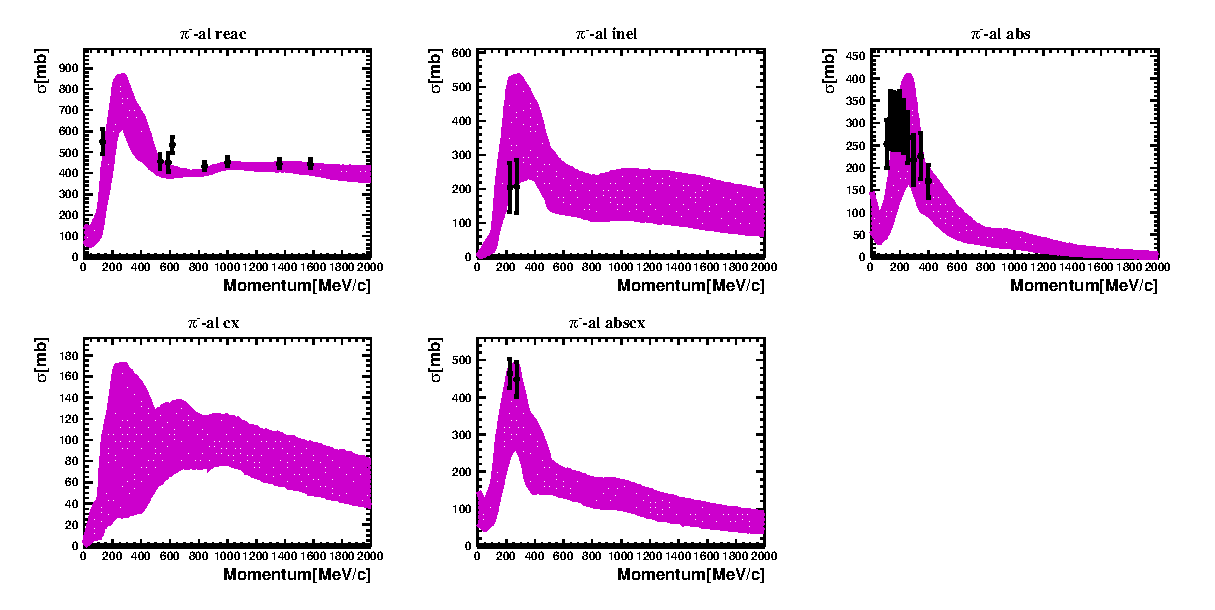
\includegraphics[width=0.9\textwidth]{T2K-TN-254/images/systematics/al_piM_all.eps}
  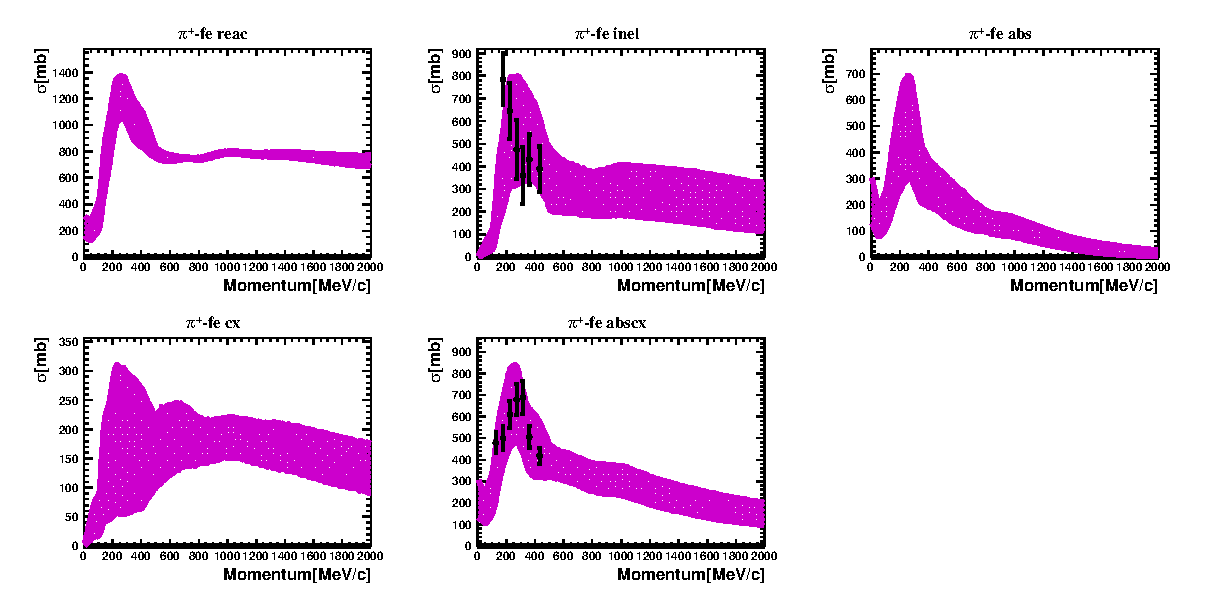
\includegraphics[width=0.9\textwidth]{T2K-TN-254/images/systematics/fe_piP_all.eps} 
  \caption[Comparison of pion scattering data to NEUT prediction and
  uncertainty]{Comparison of pion scattering data to \Gls{NEUT}
    prediction and uncertainty.  \textbf{\textit{Top five:}}
    Negatively charged pion on aluminium.  \textbf{\textit{Bottom
        five:}} Positively charged pion on iron.  From~\cite{FSITalk},
    for references, see in Table~(5.1) of~\cite{TN033}.}
  \label{fig:fsiheavy}
\end{figure}
\clearpage

\subsection{Effects on the selection}

The effects from the nucleon level pion production uncertainties are
shown in Figure~\ref{fig:infvpiproduncertainty}, which shows the
effects on the number of selected events for \Gls{FGD}1 \Gls{FV}
events only. Note that the \Gls{NC} coherent weight distribution shows
a spike at 45 events which corresponds to no coherent events in the
selection. Since the uncertainty is a Gaussian function centred at one
with an error of one; this is expected to happen 16\% of the time.

\begin{figure}[ht]
  \begin{adjustbox}{center}
    \includegraphics[width=0.8\textwidth]{images/NCg/PiProd.pdf} 
  \end{adjustbox}
  \center
  \caption[Effects of the pion resonant cross section uncertainties on
  the number of selected events]{Effects of the pion resonant cross
    section uncertainties on the number of selected events. The
    nominal central value is indicated by the black arrow.}
  \label{fig:infvpiproduncertainty}
\end{figure}

The other \Gls{CCQE} and \gls{nue} cross section errors effects are
shown in Figure~\ref{fig:infvotheruncertainty}.

\begin{figure}[ht]
  \center
  \includegraphics[width=0.8\textwidth]{images/NCg/Other_Jon.pdf} 
  \caption[Effects of the DIS (CC and NC), CCQE, CC coherent and nue
  cross section uncertainty on the number of selected events]{Effects
    of the \Gls{DIS} (\Gls{CC} and \Gls{NC}), \Gls{CCQE}, \Gls{CC}
    coherent and \gls{nue} cross section uncertainty on the number of
    selected events. The nominal central value is indicated by the
    arrow.}
  \label{fig:infvotheruncertainty}
\end{figure}


%%% Local Variables:
%%% mode: latex
%%% TeX-master: Thesis
%%% End:

\clearpage

\section{Detector systematic uncertainties}
\label{sec:detsyst}

The motivation for each of the detector uncertainty is detailed here.
There are three ways of implementing the \Gls{ND} detector systematic
uncertainties in \Gls{TK}, the first ones are called ``variation
systematics'', where the physical quantity (momentum and \Gls{TPC}
\Gls{PID} pull) that is being measured is changed according to the
effect of the systematic; another type controls the normalisation of a
whole class of events (so-called ``normalisation-like systematics'')
and finally, ``efficiency-like systematics'' which control, on an
event by event basis the weight of an event. All the uncertainties
that comes from detector effects are described here.

\subsection{Variation systematic uncertainties}

\subsubsection{The momentum scale uncertainty}
\label{subsec:momscale}
The magnetic field has an absolute error of $0.57\%$ that gets
directly propagated on the momentum of the particle~\cite{TN212}.

\subsubsection{The magnetic~/~electric field uncertainty}
\label{subsubsec:bfield}
The magnetic and electric field uncertainty~\cite{TN212} comes from
the fact that both the fields are not uniform in the \Gls{TPC}. This
is due to the presence of various equipment around the \Gls{TPC} or
the \Gls{TPC} case itself which produce fringe fields. In general, the
magnetic field and these fringe fields make the drift electrons from
the ionisation travel in a line which is not straight, which makes the
reconstruction more complicated. Some corrections can be applied at
the reconstruction level to take this effect into account, but there
is still a systematic uncertainty which has applied to the
reconstructed momentum.

On the cathode, some ``dots'' can be illuminated by lasers to produce
photo-electrons. These electrons drift until the readout plane, and
one can estimate the error on the corrections by calculating distance
from the reconstructed position of the dots to their real position.
This leads, at the analysis level, to an uncertainty on the momentum
of the particle.

\subsubsection{The momentum resolution uncertainty}
\label{subsec:momresol}
The \Gls{TPC} momentum resolution~\cite{TN212} was computed with
through going tracks that are reconstructed in multiple
\Glspl{TPC}. This systematic uncertainty aims at characterising the
intrinsic momentum resolution of the \Glspl{TPC}. The presence of
intermediate \Glspl{FGD} complicates the error calculation, as one
needs to correct for momentum loss in them. The uncertainty is
propagated on $1 / p_T$ where $p_T$ is the transverse momentum of the
particle (where transverse means orthogonal to the $Z$ direction, in
the $ZY$ plane). The uncertainty is around $10^{-4}$ for a
$500\text{~MeV}$ particle. This uncertainty is directly propagated on
the momentum of the particle.

\subsubsection{The \Gls{TPC} \Gls{PID} uncertainty}
\label{subsec:tpcpid}
The \Gls{PID} quantities that are used are the pulls, defined from the
$dEdx$ as shown in Equation~(\ref{eq:tpcpull}). To get an uncertainty
on these quantities, the pull is calculated for control samples on a
subset of the data available. This is then compared to the expected
\Gls{MC} distribution. In this case, the control sample is a photon
sample (electron~/~positron pairs with an invariant mass and good
\Gls{TPC} quality requirements). One obtains distributions similar to
the one shown in Figure~\ref{fig:tpcsyst} and can compare the width
and position of the Gaussian distributions which are used as
systematic uncertainties. In Figure~\ref{fig:tpcsyst}, on the right,
each of the data and \Gls{MC} distributions (in blue and green
histograms, respectively) are fitted with Gaussian functions (blue and
green curves). The \Gls{MC} predictions are then shifted to overlap
with the data by moving the mean of the Gaussian function for \Gls{MC}
and its spread, thus producing a correction that has to be applied to
the nominal \Gls{MC}.

The systematic uncertainty comes from the errors on the parameters of
the Gaussian functions, which is retrieved from the fit.

This is repeated for different momentum bin, particle type and, if the
statistics are sufficient, run period and \Gls{TPC} (in practice, this
split can only be realised for muons)~\cite{TN212}.

\begin{figure}[ht]
  \center
  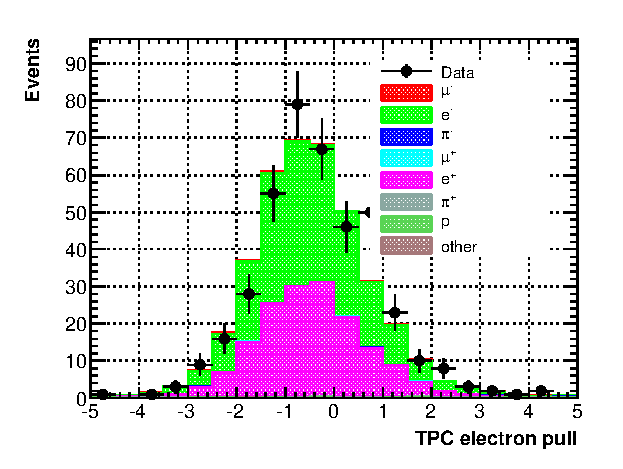
\includegraphics[width=0.48\textwidth]{T2K-TN-254/images/corrections/nopidcor_lowMom.eps}
  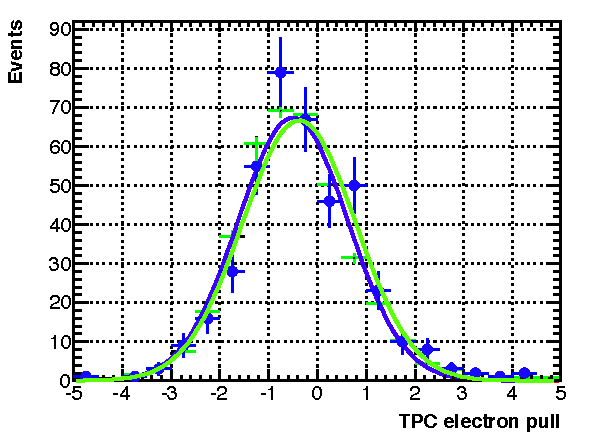
\includegraphics[width=0.48\textwidth]{T2K-TN-254/images/corrections/pidcorr_lowMom_fit.pdf}
  \caption[PID pull for electrons (or positrons) of momentum smaller
  than $200$~MeV]{\textbf{\textit{Left:}} \Gls{PID} pull for electrons
    (or positrons) of momentum smaller than $200$~MeV.
    \textbf{\textit{Right:}} \Gls{PID} pull Gaussian fits for data
    (blue) and \Gls{MC} (green).}
  \label{fig:tpcsyst}
\end{figure}


\subsection{Efficiency systematic uncertainties}
The efficiency systematic errors are applied to the events and in
general are applied to both the pair and main tracks, unless stated
otherwise.

\subsubsection{The \Gls{TPC} cluster efficiency uncertainty}
\label{subsec:tpccluster}
The \Gls{TPC} cluster efficiency uncertainty~\cite{TN212} is applied
because there is a cut on the number of nodes the tracks creates in
the \Gls{TPC} (track quality cut). Note that clusters are horizontal
or vertical hits that are joined together (see the step~2 in the
\Gls{TPC} paragraph in Section~\ref{subsubsec:reconstruction}). This
was computed by comparing the number of nodes of muon data control
samples to its equivalent in the \Gls{MC}. These control samples are a
subset of a \Gls{CC} inclusive selection and cosmic muons
triggers. The selections are run without the \Gls{TPC} track quality
and the ratios
\begin{align}
  &\frac{\epsilon_\text{Data}}{\epsilon_\text{MC}} \label{eq:effcorrection}\\
  &\text{and~}\frac{\epsilon_{\text{MC}}-\epsilon_{\text{Data}}}{\epsilon_{\text{MC}}}\label{eq:efferror}
\end{align}
are computed (in these equations, $\epsilon$ indicate the data and
\Gls{MC} efficiency). It was then found that shifts one has to apply
to the \Gls{MC} (first ratio) and error (second ratio) are both the
order of one per mil.

\subsubsection{The \Gls{TPC} track efficiency uncertainty}
\label{subsubsec:tpctrack}
The \Gls{TPC} track efficiency uncertainty~\cite{TN212} characterises
the error one gets by solely requiring the presence of a track in the
\Gls{TPC}. Rather than cluster efficiency, this error is related to
the presence of a full reconstructed object as explained in the
\Gls{TPC} paragraph of Section~\ref{subsubsec:reconstruction} (step
3). The error is computed with through-going muons which cross several
detectors. The data and \Gls{MC} comparison for such sample show that
there is no unexpected behaviour in the all \Glspl{TPC} and that the
uncertainty does not depend on the momentum, position and number of
track crossing them. The error is around $0.5\%$ for a single track
entering the \Gls{TPC}2.

\subsubsection{The \Gls{TPC}~/~\Gls{FGD} matching efficiency uncertainty}
\label{subsubsec:tpcfgdmatch}
The \Gls{TPC}~/~\Gls{FGD} matching efficiency uncertainty~\cite{TN212}
arises because the tracks in the selection have to be reconstructed as
a single object. Note that, even though there is no explicit
requirement for the Pair Track to be in the \Gls{FGD} (only a distance
specification is made), there is a priori, no requirement to apply
this error for cases where the Pair Track does not use the
\Gls{FGD}. However this was considered to be a marginal effect that
happens only if the Main Track is next to the \Gls{TPC}, on the edge
of the \Gls{FGD}, so it was applied regardless of the topology of the
Pair Track.

The efficiency was computed using through-going muons crossing
different \Glspl{TPC}, and found to be exactly $100\%$ (i.e. no track
that enter the \Gls{TPC} from the \Gls{FGD} are missed, and vice
versa). Recalling that the \Gls{FGD}1 \Gls{FV} extends to the last
layer downstream, right next to the \Gls{TPC}2, and that only two bars
are removed in the upstream direction, this is maybe not
surprising. To assign the error, it was decided that the \Gls{TPC} /
\Gls{FGD} matching could fail if a track leaves only two hits in the
\Gls{FGD} (i.e. it is very close to its edge) and therefore the hit
efficiency is used as the error, which in this case is equal to about
$0.8\%$.

\subsubsection{The \Gls{TPC}~/~\Gls{ECal} matching efficiency uncertainty}
\label{subsubsec:tpcecalmatch}
It was found recently that the \Gls{ECal}'s representation in the
\Gls{MC} was few millimetres away from its real position. Therefore
there could be a mismatch between the probability in reconstructing a
particle in the \Gls{ECal} which came from the \Gls{TPC} in data and
\Gls{MC}. This could affect the \Gls{ECal} veto since there is a
requirement for the selected veto object to not be one of the two
tracks. An uncertainty is therefore applied on the \Gls{MT} of
\Gls{PT} when they enter the \Gls{ECal}. The uncertainty which is
propagated on these tracks is of the order of $5\%$~\cite{TN279}.

\subsubsection{Charge Identification uncertainty}
\label{subsubsec:chargeid}
The charge identification is a fundamental input to the analysis,
since it relies on the selection of two tracks of opposite charge.
The error that is used is determined from the control samples which
have a muon traversing several \Glspl{TPC}~\cite{TN212}. One can then
compare the probability to incorrectly swap the charge between data
and \Gls{MC}. The error decreases with the number of \Gls{TPC} the
particle traverses; in the worst case, when the track is reconstructed
in two \Glspl{TPC}, and each one reconstructs a different charge, the
uncertainty is of $2\%$.  The error is propagated on the inverse
transverse momentum as in the case of the momentum resolution.

\subsection{Normalisation uncertainties}
These uncertainties are applied to a whole class of events based on
their topologies, it generally does not rely on the detector
efficiencies themselves, but rather on other effects such as the cross
section (for the pion and proton secondary interaction), the mass
uncertainties (for the photon secondary interactions and the \Gls{FGD}
mass), or the presence of additional events (pile up uncertainties).

\subsubsection{\Gls{FGD} mass uncertainty}
\label{subsec:fgdmass}
The \Gls{FGD} has a mass uncertainty of $0.6\%$, which comes from the
uncertainty in size of its bars and the hole for the
fibre~\cite{TN212}.

\subsubsection{The pile up and sand uncertainties}
\label{subsec:pileup}
The pile up uncertainty comes from the fact that vetoes are present in
the selection. Indeed, additional ``\gls{sand}'' events that comes
from the sand around the \Gls{ND} can reach the detector and trigger
the veto of the selection. In the interest of time and space, these
events are not included in the standard ``\gls{magnet} \Gls{MC}''
(i.e. events that are in happening the volume enclosed by the \Gls{ND}
magnet) that is used for the analysis, they are added separately. The
problem is then, since these ``\gls{sand}'' events are added
separately on top of the simulation, how to see their effect on the
vetoes? For example, if a ``\gls{magnet}'' event is selected and
passes the selection, and if there was a ``\gls{sand}'' in the same
time, one would expect to select fewer events. Hence the name, the
magnet and sand events are ``piled up.''

The way to overcome this is by calculating a pile up correction and
uncertainty. For that, the strategy is to run a selection which only
has the vetoes, and comparing the data to the sum of the \gls{magnet}
\Gls{MC} and \gls{sand} \Gls{MC}. The vetoes are added in the same
order as in the selection.

Note that the \gls{sand} events have an intrinsic uncertainty of
$10\%$, which comes from the simulation of the surroundings of the
\Gls{ND}, the flux uncertainty and the cross section.

Upon assigning the pile up correction, the strategy is to modify the
normalisation of the whole selection based on the \gls{sand} trigger
rate one gets. The error is either the data~/~\Gls{MC} difference, or
the \gls{sand} error if it is greater than the former. All the errors
and corrections are listed in Table~\ref{tab:pileup}, note that the
correction is dependent on the run, since the \Gls{MR} power increases
and produces different yields in the vetoes due to the expected
increase in \gls{sand} interaction and thus pile up.

\begin{table}[ht]
  \center
  \begin{tabular}{cccc}
    \toprule
    Veto & Run & Correction & Systematic uncertainty \\
    \cmidrule(r){1-4}
    \multirow{6}{*}{\Gls{TPC} muon rejection} & 2A  & 0.992 & 0.009 \\
         & 2W  & 0.993 & 0.007 \\
         & 3AB & 0.994 & 0.009 \\
         & 3AC & 0.991 & 0.009 \\
         & 4A  & 0.989 & 0.010 \\
         & 4W  & 0.990 & 0.010 \\
    \cmidrule(r){1-4}                        
    \multirow{6}{*}{\Gls{TPC} Veto} & 2A  & 0.995 & 0.008 \\
         & 2W  & 0.996 & 0.007 \\
         & 3AB & 0.996 & 0.008 \\
         & 3AC & 0.994 & 0.009 \\
         & 4A  & 0.992 & 0.010 \\
         & 4W  & 0.994 & 0.010 \\
    \cmidrule(r){1-4}                        
    \multirow{6}{*}{\Gls{PD} Veto} & 2A  & 0.928 & 0.009 \\
         & 2W  & 0.936 & 0.008 \\
         & 3AB & 0.937 & 0.009 \\
         & 3AC & 0.920 & 0.010 \\
         & 4A  & 0.897 & 0.012 \\
         & 4W  & 0.906 & 0.010 \\
    \cmidrule(r){1-4}
    \multirow{6}{*}{\Gls{ECal} Veto} & 2A  & 0.9989 & 0.0006 \\
         & 2W  & 0.9983 & 0.0007 \\
         & 3AB & 0.9991 & 0.0007 \\
         & 3AC & 0.9979 & 0.0008 \\
         & 4A  & 0.9974 & 0.0008 \\
         & 4W  & 0.9967 & 0.0010 \\

    \bottomrule
  \end{tabular}
  \caption[Pile up corrections and systematic uncertainties used in
  the analysis]{Pile up corrections and systematic uncertainties used
    in the analysis.}
  \label{tab:pileup}
\end{table}

Finally, as no \gls{sand} event enters the actual selection, they thus
lead to no additional uncertainty.

\subsubsection{The pion secondary interaction uncertainty}
\label{subsec:pionsec}
The pion secondary interaction uncertainty~\cite{TN212} is a weight
error that is propagated on the events which have charged pions in
them. A secondary interaction happens when this pion reinteracts with
some of the detector material, rather than losing energy by ionisation
in the detector.

There are a lot of channels in which a charged pion can interact, but
the most important in the context of this analysis is the charge
exchange channel, where a pion goes from being a charged pion to a
neutral pion after interaction with a nucleus. Unfortunately, the
\Gls{MC} model that was implemented in the \Gls{ND} simulations
(Bertini model~\cite{WRIGHT2015175}) was found to very poorly describe
the available data at \Gls{TK}
energies~\cite{TN125,TN325,Ashery:1981tq} ($200\text{~MeV}$);
therefore a correction factor was included in the cross section for
charged pions. The error on the above mentioned
data~\cite{Ashery:1981tq} was also propagated to the weight to be able
to get an uncertainty on the secondary pion interaction. Note that
these are completely uncorrelated with the \Gls{FSI} errors as
described earlier; correlating the pion secondary interaction and the
\Gls{FSI} will constitute an improvement for the next generation of
analyses at the \Gls{ND}.

\subsubsection{The proton secondary interaction uncertainty}
\label{subsec:protonsec}
The proton secondary interaction probability uncertainty~\cite{TN212}
is propagated if the \Gls{MT} or \Gls{PT} is a proton. This happens if
the \Gls{PID} did not work properly, for example. The low energy
protons have a probability of interacting with the scintillator in the
\Gls{FGD} and can reinteract in it. A very conservative error of
$10\%$ is applied for the proton interactions.

\subsubsection{The photon secondary interaction uncertainty}
\label{subsec:photonsec}
\input{T2K-TN-313/systematicsoofv.tex}

\subsubsection{Out of fiducial volume reconstruction uncertainty}
\label{subsec:recooofv}
This uncertainty is propagated because the \Gls{MT} and \Gls{PT} are
selected inside the \Gls{FV} of the detector. This was based on work
from~\cite{TN098}. It can happen that the tracks come from outside the
fiducial volume but are reconstructed inside if for example there was
a failure to detect a hit in the outer layers of the \Gls{FGD}, or a
hard scatter in the \Gls{FGD} that somehow confuses the
reconstruction. These can sometime have a large uncertainty ($30$ to
$50\%$) depending on the topology of the track.


\subsection{Summary of the detector uncertainties}
\label{subsec:detsystsummary}

Table~\ref{tab:detectoruncertaintyinfv} gives a summary of the overall
effects of all the detector errors. Note that in this table, the
positive and negative errors are determined using the \Gls{HPD}
(Highest Posterior Density) method\footnote{The following method was
  used to calculate the error of a distribution:
  \begin{itemize}[noitemsep,topsep=0pt]
  \item Find the mode of the distribution, which is now referred as
    $N_\text{event}^\text{mode}$,
  \item Create an interval for which the \Gls{PDF} is constant and
    contain the $68\%$ of the total distribution,
  \item Read off the values corresponding to the number of events (on
    the X axis) the positive and negative values are called
    $N_\text{event}^{\pm}$,
  \item Use the values
    $\frac{\left|N_\text{event}^\text{mode} -
        N_\text{event}^\pm\right|}{N_\text{event}^\text{mode}}$ as the
    positive and negative relative uncertainties. \label{ftn:hpd}
  \end{itemize}
}. Note that this method is quite sensitive to the number of toy
thrown and the binning chosen for the computation.

Figure~\ref{fig:detectorsystematicsinfv} shows the \Gls{PDF} of the
selected event after propagation of the detector errors.

\begin{table}[ht]
  \center
  \begin{tabular}{ll}
    \toprule
    Systematic & Relative uncertainty \\
    \midrule
    \multicolumn{2}{l}{Weight errors} \\
    \midrule
    Charge identification efficiency         & 0.002  \\
    \Gls{TPC} cluster efficiency             & 0.000009\\
    \Gls{TPC} track efficiency               & 0.011  \\
    \Gls{TPC}~/~\Gls{FGD} matching efficiency& 0.006  \\
    \Gls{TPC}~/~\Gls{ECal} matching efficiency & $< 0.00001$  \\
    \Gls{FGD} mass                           & 0.043  \\
    Secondary interaction pion               & 0.046  \\
    Secondary interaction proton             & 0.026  \\
    Secondary interaction photon             & $\pm^{0.41}_{0.15}$  \\
    Reconstructed \Gls{OOFV}                 & 0.061  \\
    \Gls{ECal} pile up                       & 0.0004 \\
    Muon rejection pile up                   & 0.0004  \\
    \Gls{PD} pile up                         & 0.006  \\
    \Gls{TPC} pile up                        & 0.005  \\
    \midrule
    \multicolumn{2}{l}{Variation errors} \\
    \midrule
    Magnetic field      & 0.009 \\
    Momentum scale      & 0.022 \\
    Momentum resolution & 0.025 \\
    \Gls{TPC} \Gls{PID} & 0.019 \\
    \midrule
    Total & $\pm^{1.24}_{0.20}$ \\
    \bottomrule
  \end{tabular}
  \caption[Detector uncertainties for the selected events]{Relative
    detector uncertainties for the events that pass the selection.}
  \label{tab:detectoruncertaintyinfv}
\end{table}

\begin{figure}[ht]
  \center
  \includegraphics[width=0.8\textwidth]{images/NCg/Det.pdf} 
  \caption[Effect of the detector uncertainty on the number of
  selected events]{Effect of the detector uncertainty on the number of
    selected events. The nominal central value is indicated by the
    arrow.}
  \label{fig:detectorsystematicsinfv}
\end{figure}


%%% Local Variables:
%%% mode: latex
%%% TeX-master: "Thesis"
%%% End:

\clearpage

\section{Total uncertainty}
\label{sec:totaluncertainty}


\subsection{Statistical uncertainty}
\label{subsec:statuncertainty}
To account for statistical uncertainty, the data normalisation was
thrown according to a Poisson distribution of parameter the number
events expected. Similarly, for the \Gls{MC} statistic uncertainty,
same procedure was applied without any weight nor correction or
tuning. Doing this, one finds that the relative statistical
uncertainty is \datastaterror for the data, and \mcstaterror for the
\Gls{MC}. The effect on the selected events is shown in
Figure~\ref{fig:statuncertainty}.

\begin{figure}[ht]
  \begin{adjustbox}{center}
    \includegraphics[width=0.8\textwidth]{images/NCg/stat.pdf}
  \end{adjustbox}
  \caption[Effect of all the statistical uncertainties on the number
  of selected events]{Effect of all the statistical uncertainties
    (data and \Gls{MC}) on the number of selected events. The nominal
    central value is indicated by the arrow.}
  \label{fig:statuncertainty}
\end{figure}

\subsection{Efficiency uncertainty}
\label{subsec:effuncertainty}
The efficiency also has an systematic error associated to it. To get
it, the statistical uncertainty on the number of events selected after
all the cuts is computed (simply the square root of the number of
event divided by the number of event selected).  To do this, a very
high \Gls{POT} of \Gls{NCg} events have been generated
($6.5\times 10^{24}$ \Gls{POT}).

\subsection{Combination of asymmetric error}
\label{subsec:combinationerror}
To combine all the systematic errors and get a toy distribution
allowing a proper treatment of the very asymmetric detector error that
was discussed in the previous sections, a ``discrete convolution
method'' was proposed, this method is now described.

All the independent errors were thrown, including the Poisson
statistical uncertainty of the data and MC. In a standard cross
section analysis where all the errors that are Gaussian, the errors
are then added in quadrature and get the number of event at 90\%
\Gls{CL}, $N_\text{events}^{90\%CL}$, by integrating:
\begin{equation}
\label{eq:integral}
0.90 = \int^{N_\text{events}^{90\%\text{CL}}}_{-\infty}\text{Gauss}\left(\mu = N_\text{events}^\text{nominal}, \sigma \right) dN_\text{events},
\end{equation}
where $N_\text{events}^\text{nominal}$ is the nominal number of events
after all the correction and tuning, and $\sigma$ is the total
uncertainty on this number after summing all the independent errors in
quadrature.

Note that the assumption that one can add the errors in quadrature is
central in this method. However, it cannot be applied for asymmetric
errors as is the case in this analysis.

Rather than adding the errors in quadrature, the ratios
$N_\text{events}^\text{toy} / N_\text{event}^\text{nominal}$ were
computed for each toy and for each uncertainty source. To get the
total \Gls{PDF} (Probability Distribution Function) of the number of
selected events, one just has to multiply all these ratios with each
other:
\begin{equation}
\label{eq:toycombination}
N_\text{events}^\text{toy} = N_\text{event}^\text{nominal} \times \prod_{i = \text{source}}\prod_{j = \text{toy}}
\frac{N_\text{events}^{\text{toy} i,j}}{N_\text{events}^\text{nominal}},
\end{equation}
where $i$ denotes the source of the uncertainty (it can be detector,
flux, \Gls{FSI}, cross section, data or \Gls{MC} statistics), and $j$
is the particular toy. In practice, the number of toy experiments
grows exponentially with the number of source of systematic errors,
therefore the systematic uncertainties with Gaussian behaviour (flux,
cross section, \Gls{FSI}, data and \Gls{MC} statistics) were added in
quadrature and used to generate 1000 toy experiments to combine with
the asymmetric detector uncertainty as described earlier.

\subsection{Effect of all uncertainties}
When combining the uncertainties as described in the previous section,
one obtains the distribution shown in Figure~\ref{fig:allsyst}.

\begin{figure}[ht]
  \begin{adjustbox}{center}
    \includegraphics[width=0.8\textwidth]{images/NCg/All.pdf}
  \end{adjustbox}
  \caption{Effect of all the uncertainties in the total number of
    selected events.}
  \label{fig:allsyst}
\end{figure}

Note, that as can be seen in Figure~\ref{fig:detectorsystematicsinfv},
the detector systematic uncertainties introduce a relatively large
bias towards higher number of events. This bias gets propagated on the
total systematic uncertainty distribution (``All errors'' on
Figure~\ref{fig:allsyst}), but not on the other distributions (cross
section errors, \Gls{FSI}, flux). This is why the error on pion
production \Gls{PDF} seems to extend towards lower number of events
than the one with all the errors. It was checked that appling the same
bias to the pion production error gives shifts the pion production
error \Gls{PDF} under the one with all the errors.

\subsection{\texorpdfstring{Motivation of the $\varphi_\text{photon}$ cut}%
  {Motivation of the photon phi cut}}
\label{subsec:downwardphotons}

An interesting feature is exhibited in Appendix~\ref{app:mass}, for
bottom-originated events, there is a higher uncertainty than for the
rest of the selection (Table~\ref{tab:oofvmasserror}). Since the
pointing capabilities of the \Gls{FGD}1 is reasonably good for event
coming from all the directions (see Appendix~\ref{app:rec}), one can
restrict the phase space to events originated from the top and the
side directions. This is done with a simple cut on the $\varphi$ angle
of the reconstructed photon direction.  The effect of adding this
phase space cut is shown in Figure~\ref{fig:detectorphi}.

However, such a cut would have an impact too drastic on the efficiency
and on the statistics of the selected events. So, rather than removing
all the events from the downward direction, the cut was optimised. To
do that, the only uncertainties of interest are the detector
systematic errors and the data statistical error. Similarly, the
efficiency is going to decrease if one removes too many events from
downward. The optimisation of this cut was performed by minimising its
value by minimizing the value $N_\text{Signal}/\epsilon$

In this ratio, $N_\text{Signal}$ is the difference between the 90\%
upper \Gls{CL} of the number of \Gls{MC} events and the nominal number
of events (which essentially gives an idea of the uncertainty) and
$\epsilon$ is the efficiency. The Figure~\ref{fig:optimisationphi}
motivates the chosen value of $\varphi_\text{cut} = 36^{\circ}$. This
value is then translated for the excluded angles
$\varphi_{\text{photon}}$:

\begin{align}
  -90^{\circ} - \varphi_{\text{cut}} / 2 &< \varphi_{\text{photon}} < -90^{\circ} + \varphi_{\text{cut}} / 2 \\
  -108^{\circ} & <  \varphi_{\text{photon}} < -72^{\circ}.
\end{align}

All the errors are depicted in Figure~\ref{fig:allsystphi} and
summarised in Table~\ref{tab:AllErrorPhiCut} after this cut (called
$\varphi_\text{photon}$ cut from now on). Note that in this table, the
positive and negative errors are determined using the \Gls{HPD}
(Highest Posterior Density) method (see Footnote~\ref{ftn:hpd} on
page~\pageref{ftn:hpd}). As explained earlier, this method is quite
sensitive to the number of toy thrown and the binning chosen for the
computation. For example, it fails in giving a reasonable answer for
the \Gls{COH} cross section error, since the highest probability is at
the edge of its \Gls{PDF}. Therefore, only the detector and the total
errors have been computed using this method.

\begin{figure}[ht]
  \begin{adjustbox}{center}
    \includegraphics[width=0.8\textwidth]{T2K-TN-254/images/systematics/QuantilePhiBTZ.pdf} 
  \end{adjustbox}
  \caption[PDF of the selected number of events from the detector
  uncertainties after the azimuthal cut ($\varphi > 0$)]{\Gls{PDF} of
    the selected number of events from detector uncertainties
    (including the \Gls{OOFV} one) after the azimuthal cut
    ($\varphi > 0$). The nominal central value is indicated by the
    arrow.}
  \label{fig:detectorphi}
\end{figure}

\begin{figure}[ht]
  \begin{adjustbox}{center}
    \includegraphics[width=0.8\textwidth]{T2K-TN-254/images/systematics/Optimisation.pdf} 
  \end{adjustbox}
  \caption[Optimisation of the $\varphi$ cut]{Optimisation of the
    $\varphi$ cut, showing the contribution of the data statistic,
    detector systematic errors and efficiency on
    $N_\text{Signal}/\epsilon$, which is proportional to the cross
    section limit.}
  \label{fig:optimisationphi}
\end{figure}

\begin{figure}[ht]
  \begin{adjustbox}{center}
    \includegraphics[width=0.8\textwidth]{T2K-TN-254/images/systematics/QuantilePhi.pdf} 
  \end{adjustbox}
  \caption[PDF of the selected number of events from the detector
  uncertainties after the optimised azimuthal cut (with events
  satisfying $-108^{\circ} < \varphi_{\text{photon}} < -72^{\circ}$
  excluded)]{\Gls{PDF} of the selected number of events from the
    detector uncertainties after the optimised azimuthal cut (with
    events satisfying
    $-108^{\circ} < \varphi_{\text{photon}} < -72^{\circ}$ excluded).
    The nominal central value is indicated by the arrow. The $90\%$
    quantile of the \Gls{MC} is also shown.}
  \label{fig:allsystphi}
\end{figure}

\begin{table}[ht]
  \begin{adjustbox}{center}
    \begin{tabular}{lc}
      \toprule
      Systematic error &Relative uncertainty \\ 
      \midrule
      Statistical error on Data (expected) & $\pm 0.14$ \\ 
      Statistical error on Data (observed) & $\pm 0.16$ \\ 
      Statistical error on \Gls{MC}        & $\pm 0.032$ \\ 
      \midrule
      Detector errors                      & $\pm^{0.27}_{0.17}$\\ 
      \midrule
      $C_{A}^{5}$ \Gls{RES} error              &$\pm0.078$ \\ 
      $M_{a}$ \Gls{RES} error                 &$\pm0.089$ \\ 
      Background scale \Gls{RES} error        &$\pm0.023$\\ 
      Nuclear \Gls{RES} ($\Delta$ mass) error &$\pm0.002$\\ 
      \midrule                                
      All errors on single pion production    &$\pm0.20$\\ 
      \midrule
      \Gls{CCQE} errors        & $\pm 0.003 $\\ 
      \Gls{CC}\Gls{nue} error  & $\pm 0.006 $\\ 
      \Gls{DIS} error          & $\pm 0.012 $\\ 
      \Gls{CC} \Gls{COH} error & $\pm 0.001 $\\ 
      \Gls{NC} \Gls{COH} error & $\pm 0.163 $\\ 
      Other \Gls{NC} error     & $\pm 0.032 $\\ 
      \midrule
      All cross section errors (except single pion production) & $\pm 0.036$\\ 
      \midrule
      Flux error & $\pm 0.082$\\ 
      \midrule
      \Gls{FSI} error & $\pm 0.037$\\
      \midrule
      Efficiency error & $\pm 0.0985$ \\
      \midrule
      All errors (except efficiency) & $\pm^{0.33}_{0.23}$ \\ 
      \bottomrule
    \end{tabular}
  \end{adjustbox}
  \caption[Summary of all the errors after the $\varphi$ angle
  cut]{Summary of all the errors after the $\varphi$ angle cut using
    the \Gls{HPD} method.}
  \label{tab:AllErrorPhiCut}
\end{table}


\subsection{Conclusion}
In this section, the importance of each systematic uncertainty and its
effect on the number of selected events were shown. In the case of a
analysis which aims to set a limit, careful characterisation of the
systematic uncertainties is primoridial. This is because the limit is
directly proportional to the total systematic errors (at least in the
case of Gaussian errors). All the asymmetric errors were added
coherently via the described method of discrete convolution. The main,
dominant, error is the detector uncertainty. This error is mitigated
by adding a cut on the reconstructed azimuthal angle of the photon and
removing the photons that comes from under the \Gls{ND}, which have a
large propagation error.

%%% Local Variables:
%%% mode: latex
%%% TeX-master: "Thesis"
%%% End:

\clearpage


%%% Local Variables:
%%% mode: latex
%%% TeX-master: "Thesis"
%%% End:
